\begin{task}
    
\TT{Wyznacz współczynniki zespolonego szeregu Fouriera dla okresowego sygnału $f(t)$ przedstawionego na rysunku. Wykorzystaj więdzę o liniowości szeregu Fouriera i o wpływie przesunięcia sygnału w czasie na współczynniki szeregu Fouriera.}{Calculate coefficients of the periodic signal $f(t)$ shown below for the expansion into a complex exponential Fourier series. Use knowledge about linearity of complex exponential Fourier series and about the effect of signal shift in time on the complex exponential Fourier series.}

\begin{figure}[H]
\centering
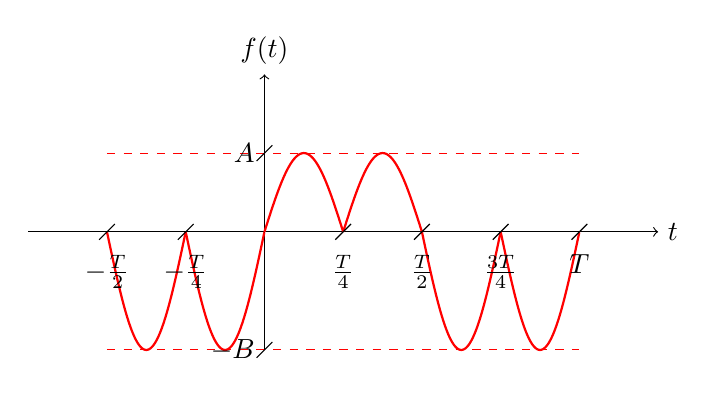
\begin{tikzpicture}
  %\draw (0,0) circle (1in);
  \draw[->] (-3.0,+0.0) -- (+5.0,+0.0) node[right] {$t$};
  \draw[->] (+0.0,-1.5) -- (+0.0,+2.0) node[above] {$f(t)$};
  \draw[scale=1.0,domain=-2.0:-1.0,samples=100,smooth,variable=\x,red,thick] plot ({\x},{0.0-1.5*sin(\x*180.0)});
  \draw[scale=1.0,domain=-1.0:0.0,samples=100,smooth,variable=\x,red,thick] plot ({\x},{0.0+1.5*sin(\x*180.0)});
  \draw[scale=1.0,domain=0.0:1.0,samples=100,smooth,variable=\x,red,thick] plot ({\x},{0.0+1.0*sin(\x*180.0)});
  \draw[scale=1.0,domain=1.0:2.0,samples=100,smooth,variable=\x,red,thick] plot ({\x},{0.0-1*sin(\x*180.0)});
  \draw[scale=1.0,domain=2.0:3.0,samples=100,smooth,variable=\x,red,thick] plot ({\x},{0.0-1.5*sin(\x*180.0/3.141592*1*3.141592/1.0)});
  \draw[scale=1.0,domain=3.0:4.0,samples=100,smooth,variable=\x,red,thick] plot ({\x},{0.0+1.5*sin(\x*180.0/3.141592*1*3.141592/1.0)});
  \draw[-,red, dashed] (-2.0,1.0) -- (4.0,1.0);
  \draw[-,red, dashed] (-2.0,-1.5) -- (4.0,-1.5);
  \draw[-] (-2.0-0.1,-0.1)--(-2.0+0.1,0.1) node[midway, below, outer sep=5pt] {$-\frac{T}{2}$};
  \draw[-] (-1.0-0.1,-0.1)--(-1.0+0.1,0.1) node[midway, below, outer sep=5pt] {$-\frac{T}{4}$};
  \draw[-] (+1.0-0.1,-0.1)--(+1.0+0.1,0.1) node[midway, below, outer sep=5pt] {$\frac{T}{4}$};
  \draw[-] (+2.0-0.1,-0.1)--(+2.0+0.1,0.1) node[midway, below, outer sep=5pt] {$\frac{T}{2}$};
  \draw[-] (+3.0-0.1,-0.1)--(+3.0+0.1,0.1) node[midway, below, outer sep=5pt] {$\frac{3T}{4}$};
  \draw[-] (+4.0-0.1,-0.1)--(+4.0+0.1,0.1) node[midway, below, outer sep=5pt] {$T$};
  \draw[-] (-0.1,+1.0-0.1)--(+0.1,+1.0+0.1) node[midway, left] {$A$};
  \draw[-] (-0.1,-1.5-0.1)--(+0.1,-1.5+0.1) node[midway, left] {$-B$};

\end{tikzpicture}
\end{figure}

\TT{W pierwszej kolejności należy ustalić wzór funkcji przedstawionej na rysunku. Jest to funkcja odcinkowa, którą możemy opisać w następujący sposób:}{First of all, the definition of $f(t)$ signal has to be derived. This is periodic piecewise function, which may be describe as:}

\begin{equation}
f(t)=\begin{cases}A \cdot sin\left( \frac{4\pi}{T} \cdot t\right) & t \in \left ( 0+k \cdot T; \frac{T}{4}+k \cdot T \right ) \\
-A \cdot sin\left( \frac{4\pi}{T} \cdot t\right) & t \in \left ( \frac{T}{4}+k \cdot T; \frac{T}{2}+k \cdot T \right ) \\
-B \cdot sin\left( \frac{4\pi}{T} \cdot t\right) & t \in \left ( \frac{T}{2}+k \cdot T; \frac{3T}{4}+k \cdot T \right )\\
B \cdot sin\left( \frac{4\pi}{T} \cdot t\right) & t \in \left ( \frac{3T}{4}+k \cdot T; T+k \cdot T \right )
\end{cases} \wedge k \in \TT{C}{Z}
\end{equation}

\TT{Współczynniki $F_k$ możemy wzynaczyć bezpośrednio z definicji. Ponieważ mamy sygnał okresowy, w którym każdy okres składa się z czterech odcinków, to trzeba będzie obliczyć po jednej całce dla każdego z odcinków. Można również zauważyć, że sygnał $f(t)$ da się przedstawić jako liniową kombinację poprzesuwanego w czasie sygnału $g(t)$ przedstawionego poniżej:}{The $F_k$ coefficients may be calculated directly by definition. However, four integrals have to be solved, each for single interval of one period of the $f(t)$ signal. If we look carefully, signal $f(t)$ may be decomposed into linear combination of shifted in time $g(t)$ signals, for $g(t)$ signal given below:}

\begin{figure}[H]
    \centering
    \begin{tikzpicture}
    %\draw (0,0) circle (1in);
    \draw[->] (-3.0,+0.0) -- (+5.0,+0.0) node[right] {$t$};
    \draw[->] (+0.0,-1.5) -- (+0.0,+2.0) node[above] {$g(t)$};
    \draw[-,red,thick] (-2.0,0.0) -- (+0.0,+0.0);
    \draw[scale=1.0,domain=0.0:1.0,samples=100,smooth,variable=\x,red,thick] plot ({\x},{0.0+1.0*sin(\x*180.0)});
    \draw[-,red,thick] (1.0,0.0) -- (+4.0,+0.0);
    \draw[-,red, dashed] (-2.0,1.0) -- (4.0,1.0);
    \draw[-,red, dashed] (-2.0,-1.5) -- (4.0,-1.5);
    \draw[-] (-2.0-0.1,-0.1)--(-2.0+0.1,0.1) node[midway, below, outer sep=5pt] {$-\frac{T}{2}$};
    \draw[-] (-1.0-0.1,-0.1)--(-1.0+0.1,0.1) node[midway, below, outer sep=5pt] {$-\frac{T}{4}$};
    \draw[-] (+1.0-0.1,-0.1)--(+1.0+0.1,0.1) node[midway, below, outer sep=5pt] {$\frac{T}{4}$};
    \draw[-] (+2.0-0.1,-0.1)--(+2.0+0.1,0.1) node[midway, below, outer sep=5pt] {$\frac{T}{2}$};
    \draw[-] (+3.0-0.1,-0.1)--(+3.0+0.1,0.1) node[midway, below, outer sep=5pt] {$\frac{3T}{4}$};
    \draw[-] (+4.0-0.1,-0.1)--(+4.0+0.1,0.1) node[midway, below, outer sep=5pt] {$T$};
    \draw[-] (-0.1,+1.0-0.1)--(+0.1,+1.0+0.1) node[midway, left] {$1$};
    
    \end{tikzpicture}
\end{figure}

\TT{Jest to funkcja odcinkowa, którą możemy opisać w następujący sposób:}{This is periodic piecewise function, which may be describe as:}

\begin{equation}
g(t)=\begin{cases}sin\left( \frac{4\pi}{T} \cdot t\right) & t \in \left ( 0+k \cdot T; \frac{T}{4}+k \cdot T \right ) \\
0 & t \in \left ( \frac{T}{4}+k \cdot T; T+k \cdot T \right )
\end{cases} \wedge k \in \TT{C}{Z}
\end{equation}

\TT{Dla tak zdefiniwanego sygnału $g(t)$, sygnał $f(t)$ można przedstawić jako:}{For such a definition of $g(t)$ signal, our $f(t)$ may be described as:}

\begin{equation}
g(t)=A \cdot g\left(t\right) + A \cdot g\left(t - \frac{T}{4}\right) - B \cdot g\left(t - \frac{T}{2}\right) - B \cdot g\left(t - \frac{3T}{4}\right)
\end{equation}

\TT{Teraz wystarczy wyznaczyć współczynniki rozwinięcia w zespolony szerg Fouriera dla sygnału $g(t)$. Następnie, na podstawie twierdzenia o liniowości oraz  wpływie przesunięcia sygnału w czasie na współczynniki szeregu Fouriera będziemy mogli obliczyć współczynniki $F_k$ dla sygnału $f(t)$.}{Right now, it is enough to calculate $G_k$ - complex exponential Fourier coefficients of $g(t)$ signal. Then, based on linearity and on the effect of signal shift in time on the complex exponential Fourier series, we will be able to derive $F_k$ of $f(t)$ signal.}


\TT{Współczynnik $G_0$ wyznaczamy ze wzoru:}{The $G_0$ coefficient is defined as:}

\begin{equation}
G_0=\frac{1}{T}\int_{T}g(t) \cdot dt
\end{equation}

\TT{Podstawiamy do wzoru wzór naszej funkcji w pierwszym okresie $k=0$}{For the period $t \in (0; T)$, i.e. $k=0$, we get:}

\begin{align*}
G_0&=\frac{1}{T}\int_{T}g(t) \cdot dt=\\
&=\frac{1}{T}\left(\int_{0}^{\frac{T}{4}}sin\left( \frac{4\pi}{T} \cdot t\right) \cdot dt 
+ \frac{1}{T}\int_{\frac{T}{4}}^{T}0 \cdot dt \right)=\\
&=\frac{1}{T}\left(\int_{0}^{\frac{T}{4}}sin\left( \frac{4\pi}{T} \cdot t\right) \cdot dt 
+ 0 \right)=\\
&=\frac{1}{T}\int_{0}^{\frac{T}{4}}sin\left( \frac{4\pi}{T} \cdot t\right) \cdot dt=\\
&=\begin{Bmatrix*}[l]
z&=\frac{4\pi}{T} \cdot t\\
dz&=\frac{4\pi}{T} \cdot dt\\
dt&=\frac{dz}{\frac{4\pi}{T}}
\end{Bmatrix*}=\\
&=\frac{1}{T}\int_{0}^{\frac{T}{4}}sin\left( z\right) \cdot \frac{dz}{\frac{4\pi}{T}}=\\
&=\frac{1}{T\cdot \frac{4\pi}{T}}\int_{0}^{\frac{T}{4}}sin\left( z\right) \cdot dz=\\
&=\frac{1}{4\pi}\cdot \left(\left . -cos\left( z\right) \right|_{0}^{\frac{T}{4}}\right)=\\
&=-\frac{1}{4\pi}\cdot \left(\left . cos\left( \frac{4\pi}{T} \cdot t\right) \right|_{0}^{\frac{T}{4}}\right)=\\
&=-\frac{1}{4\pi}\cdot \left( cos\left( \frac{4\pi}{T} \cdot \frac{T}{4}\right) - cos\left( \frac{4\pi}{T} \cdot 0\right)\right)=\\
&=-\frac{1}{4\pi}\cdot \left( cos\left(\pi\right) - cos\left( 0\right)\right)=\\
&=-\frac{1}{4\pi}\cdot \left( -1 - 1\right)=\\
&=-\frac{1}{4\pi}\cdot \left( -2\right)=\\
&=\frac{1}{2\pi}
\end{align*}

\TT{Wartość współczynnika $G_0$ wynosi $\frac{1}{2\pi}$.}{The $G_0$ coefficient equals $\frac{1}{2\pi}$.}

\TT{Współczynniki $G_k$ wyznaczamy ze wzoru}{The $G_k$ coefficients are defined as:}

\begin{equation}
G_k=\frac{1}{T}\int_{T}g(t) \cdot e^{-\jmath \cdot k \cdot \frac{2\pi}{T} \cdot t} \cdot dt
\end{equation}

\TT{Podstawiamy do wzoru wzór naszej funkcji w pierwszym okresie $k=0$}{For the period $t \in (0; T)$, i.e. $k=0$, we get:}

\begin{align*}
G_k&=\frac{1}{T}\int_{T}g(t) \cdot e^{-\jmath \cdot k \cdot \frac{2\pi}{T} \cdot t} \cdot dt=\\
&=\frac{1}{T}\cdot\left(\int_{0}^{\frac{T}{4}}sin\left( \frac{4\pi}{T} \cdot t\right) \cdot e^{-\jmath \cdot k \cdot \frac{2\pi}{T} \cdot t} \cdot dt+\int_{\frac{T}{4}}^{T} 0 \cdot e^{-\jmath \cdot k \cdot \frac{2\pi}{T} \cdot t} \cdot dt\right)=\\
&=\begin{Bmatrix*}[l]
sin\left(x\right)&=\frac{e^{\jmath \cdot x}-e^{-\jmath \cdot x}}{2 \jmath }
\end{Bmatrix*}=\\
&=\frac{1}{T}\cdot\left(\int_{0}^{\frac{T}{4}} \frac{e^{\jmath \cdot \frac{4\pi}{T} \cdot t}-e^{-\jmath \cdot \frac{4\pi}{T} \cdot t}}{2\jmath} \cdot e^{-\jmath \cdot k \cdot \frac{2\pi}{T} \cdot t} \cdot dt+\int_{\frac{T}{4}}^{T} 0 \cdot dt\right)=\\
&=\frac{1}{T}\cdot\left(\frac{1}{2\jmath} \cdot \int_{0}^{\frac{T}{4}} \left(e^{\jmath \cdot \frac{4\pi}{T} \cdot t}-e^{-\jmath \cdot \frac{4\pi}{T} \cdot t}\right)\cdot e^{-\jmath \cdot k \cdot \frac{2\pi}{T} \cdot t} \cdot dt + 0\right)=\\
&=\frac{1}{T} \cdot \frac{1}{2\jmath} \cdot \int_{0}^{\frac{T}{4}}
\left( e^{\jmath \cdot \frac{4\pi}{T} \cdot t} \cdot e^{-\jmath \cdot k \cdot \frac{2\pi}{T} \cdot t} - e^{-\jmath \cdot \frac{4\pi}{T} \cdot t} \cdot e^{-\jmath \cdot k \cdot \frac{2\pi}{T} \cdot t} \right) \cdot dt=\\
&=\frac{1}{T\cdot 2\jmath} \cdot \int_{0}^{\frac{T}{4}}
\left(e^{\jmath \cdot \frac{4\pi}{T} \cdot t -\jmath \cdot k \cdot \frac{2\pi}{T} \cdot t} - e^{-\jmath \cdot \frac{4\pi}{T} \cdot t -\jmath \cdot k \cdot \frac{2\pi}{T} \cdot t} \right) \cdot dt=\\
&=\frac{1}{T\cdot 2\jmath} \cdot \int_{0}^{\frac{T}{4}}
\left(e^{\jmath \cdot \frac{2\pi}{T} \cdot t \cdot \left(2 - k\right)} - e^{-\jmath \cdot \frac{2\pi}{T} \cdot t \cdot \left(2+k\right)} \right) \cdot dt=\\
&=\frac{1}{T\cdot 2\jmath} \cdot \left( \int_{0}^{\frac{T}{4}}
e^{\jmath \cdot \frac{2\pi}{T} \cdot t \cdot \left(2 - k\right)} \cdot dt - \int_{0}^{\frac{T}{4}} e^{-\jmath \cdot \frac{2\pi}{T} \cdot t \cdot \left(2+k\right)} \cdot dt \right)=\\
&=\begin{Bmatrix*}[l]
z_1&=\jmath \cdot \frac{2\pi}{T} \cdot \left(2 - k\right)\cdot t &z_2&=-\jmath \cdot \frac{2\pi}{T} \cdot \left(2+k\right)\cdot t\\
dz_1&=\jmath \cdot \frac{2\pi}{T} \cdot \left(2 - k\right)\cdot dt &dz_2&=-\jmath \cdot \frac{2\pi}{T} \cdot \left(2+k\right)\cdot dt\\
dt&=\frac{dz_1}{\jmath \cdot \frac{2\pi}{T} \cdot \left(2 - k\right)} &dt&=\frac{dz_2}{-\jmath \cdot \frac{2\pi}{T} \cdot \left(2+k\right)}\\
\end{Bmatrix*}=\\
&=\frac{1}{T\cdot 2\jmath} \cdot \left( \int_{0}^{\frac{T}{4}}
e^{z_1} \cdot \frac{dz_1}{\jmath \cdot \frac{2\pi}{T} \cdot \left(2 - k\right)} - \int_{0}^{\frac{T}{4}} e^{z_2} \cdot \frac{dz_2}{-\jmath \cdot \frac{2\pi}{T} \cdot \left(2+k\right)} \right)=\\
&=\frac{1}{T\cdot 2\jmath} \cdot \left( \frac{1}{\jmath \cdot \frac{2\pi}{T} \cdot \left(2 - k\right)} \cdot \int_{0}^{\frac{T}{4}}
e^{z_1} \cdot dz_1 - \frac{1}{-\jmath \cdot \frac{2\pi}{T} \cdot \left(2+k\right)} \cdot \int_{0}^{\frac{T}{4}} e^{z_2} \cdot dz_2 \right)=\\
&=\frac{1}{T\cdot 2\jmath \cdot \jmath \cdot \frac{2\pi}{T} } \cdot \left( \frac{1}{2 - k} \cdot \int_{0}^{\frac{T}{4}}
e^{z_1} \cdot dz_1 + \frac{1}{2+k} \cdot \int_{0}^{\frac{T}{4}} e^{z_2} \cdot dz_2 \right)=\\
&=\frac{1}{-4 \cdot \pi} \cdot \left( \frac{1}{2 - k} \cdot \left.
e^{z_1} \right|_{0}^{\frac{T}{4}} + \frac{1}{2+k} \cdot \left. e^{z_2} \right|_{0}^{\frac{T}{4}} \right)=\\
&=\frac{1}{-4 \cdot \pi} \cdot \left( \frac{1}{2 - k} \cdot \left.
e^{\jmath \cdot \frac{2\pi}{T} \cdot \left(2 - k\right)\cdot t} \right|_{0}^{\frac{T}{4}} + \frac{1}{2+k} \cdot \left. e^{-\jmath \cdot \frac{2\pi}{T} \cdot \left(2+k\right)\cdot t} \right|_{0}^{\frac{T}{4}} \right)=\\
&=\frac{1}{-4 \cdot \pi} \cdot \left( \frac{1}{2 - k} \cdot \left(
e^{\jmath \cdot \frac{2\pi}{T} \cdot \left(2 - k\right)\cdot \frac{T}{4}} - e^{\jmath \cdot \frac{2\pi}{T} \cdot \left(2 - k\right)\cdot 0} \right) + \frac{1}{2+k} \cdot \left( e^{-\jmath \cdot \frac{2\pi}{T} \cdot \left(2+k\right)\cdot \frac{T}{4}} - e^{-\jmath \cdot \frac{2\pi}{T} \cdot \left(2+k\right)\cdot 0}\right) \right)=\\
&=\frac{1}{-4 \cdot \pi} \cdot \left( \frac{1}{2 - k} \cdot \left(
e^{\jmath \cdot \frac{\pi}{2} \cdot \left(2 - k\right)} - e^{0} \right) + \frac{1}{2+k} \cdot \left( e^{-\jmath \cdot \frac{\pi}{2} \cdot \left(2+k\right)} - e^{0}\right) \right)=\\
&=\frac{1}{-4 \cdot \pi} \cdot \left( \frac{2+k}{\left(2 - k\right)\cdot \left(2+k\right)} \cdot \left(
e^{\jmath \cdot \frac{\pi}{2} \cdot \left(2 - k\right)} - 1 \right) + \frac{2-k}{\left(2 - k\right)\cdot \left(2+k\right)} \cdot \left( e^{-\jmath \cdot \frac{\pi}{2} \cdot \left(2+k\right)} - 1\right) \right)=\\
&=\frac{1}{-4 \cdot \pi} \cdot \left( \frac{\left(2+k\right)\cdot \left(
  e^{\jmath \cdot \frac{\pi}{2} \cdot \left(2 - k\right)} - 1 \right)}{\left(2 - k\right)\cdot \left(2+k\right)} + \frac{\left(2-k\right)\cdot \left( e^{-\jmath \cdot \frac{\pi}{2} \cdot \left(2+k\right)} - 1\right)}{\left(2 - k\right)\cdot \left(2+k\right)} \right)=\\
&=\frac{1}{-4 \cdot \pi} \cdot \left( \frac{\left(2+k\right)\cdot \left(
  e^{\jmath \cdot \frac{\pi}{2} \cdot \left(2 - k\right)} - 1 \right)+\left(2-k\right)\cdot \left( e^{-\jmath \cdot \frac{\pi}{2} \cdot \left(2+k\right)} - 1\right)}{\left(2 - k\right)\cdot \left(2+k\right)} \right)=\\
&=\frac{1}{-4 \cdot \pi} \cdot \left( \frac{2 \cdot e^{\jmath \cdot \frac{\pi}{2} \cdot \left(2 - k\right)} - 2 + k\cdot e^{\jmath \cdot \frac{\pi}{2} \cdot \left(2 - k\right)} - k+ 2 \cdot e^{-\jmath \cdot \frac{\pi}{2} \cdot \left(2+k\right)} - 2 - k \cdot e^{-\jmath \cdot \frac{\pi}{2} \cdot \left(2+k\right)} + k}{4-k^2} \right)=\\
&=\frac{1}{-4 \cdot \pi} \cdot \left( \frac{2 \cdot e^{\jmath \cdot \frac{\pi}{2} \cdot \left(2 - k\right)} - 4 + k\cdot e^{\jmath \cdot \frac{\pi}{2} \cdot \left(2 - k\right)}+ 2 \cdot e^{-\jmath \cdot \frac{\pi}{2} \cdot \left(2+k\right)} - k \cdot e^{-\jmath \cdot \frac{\pi}{2} \cdot \left(2+k\right)}}{4-k^2} \right)=\\
&=\frac{1}{-4 \cdot \pi} \cdot \left( \frac{2 \cdot e^{\jmath \cdot \pi}\cdot e^{-\jmath \cdot \frac{k \cdot \pi}{2}} - 4 + k\cdot e^{\jmath \cdot \pi } \cdot e^{-\jmath \cdot \frac{k \cdot \pi}{2}}+ 2 \cdot e^{-\jmath \cdot \pi} \cdot e^{-\jmath \cdot \frac{k \cdot \pi}{2}} - k \cdot e^{-\jmath \cdot \pi}\cdot e^{-\jmath \cdot \frac{k \cdot \pi}{2}}}{4-k^2} \right)=\\
&=\begin{Bmatrix*}[l]
e^{\jmath \cdot \pi} &= cos\left(\pi\right) +\jmath \cdot sin\left(\pi\right) = -1\\
e^{-\jmath \cdot \pi} &= cos\left(\pi\right) -\jmath \cdot sin\left(\pi\right) = -1
\end{Bmatrix*}=\\
&=\frac{1}{-4 \cdot \pi} \cdot \left( \frac{2 \cdot \left(-1\right) \cdot e^{-\jmath \cdot \frac{k \cdot \pi}{2}} - 4 + k\cdot \left(-1\right) \cdot e^{-\jmath \cdot \frac{k \cdot \pi}{2}} + 2 \cdot (-1) \cdot e^{-\jmath \cdot \frac{k \cdot \pi}{2}} - k \cdot \left(-1\right)\cdot e^{-\jmath \cdot \frac{k \cdot \pi}{2}}}{4-k^2} \right)=\\
&=\frac{1}{-4 \cdot \pi} \cdot \left( \frac{-2 \cdot e^{-\jmath \cdot \frac{k \cdot \pi}{2}} - 4 - k\cdot e^{-\jmath \cdot \frac{k \cdot \pi}{2}} - 2 \cdot e^{-\jmath \cdot \frac{k \cdot \pi}{2}} + k \cdot e^{-\jmath \cdot \frac{k \cdot \pi}{2}}}{4-k^2} \right)=\\
&=\frac{1}{-4 \cdot \pi} \cdot \left( \frac{-4\cdot e^{-\jmath \cdot \frac{k \cdot \pi}{2}} - 4 }{4-k^2} \right)=\\
&=\frac{1}{4 \cdot \pi} \cdot \left( \frac{4 \cdot e^{-\jmath \cdot \frac{k \cdot \pi}{2}} +4}{4-k^2} \right)=\\
&=\frac{1}{4 \cdot \pi} \cdot 4 \cdot \left(\frac{e^{-\jmath \cdot \frac{k \cdot \pi}{2}}+1}{4-k^2} \right)=\\
&=\frac{1}{\pi} \cdot \left(\frac{1 + e^{-\jmath \cdot \frac{k \cdot \pi}{2}}}{4-k^2}\right)=\\
&=\frac{1 + e^{-\jmath \cdot \frac{k \cdot \pi}{2}}}{\pi \left(4-k^2\right)}
\end{align*}

\TT{Wartość współczynnika $G_k$ wynosi $\frac{1 + e^{-\jmath \cdot \frac{k \cdot \pi}{2}}}{\pi \left(4-k^2\right)}$ dla $k \neq 2 \wedge k \neq -2$.}{The $G_k$ coefficients are equal to $\frac{1 + e^{-\jmath \cdot \frac{k \cdot \pi}{2}}}{\pi \left(4-k^2\right)}$ for $k \neq 2 \wedge k \neq -2$.}

\TT{Współczynnik $G_k$ dla $k=2$ musimy wyznaczyć raz jeszcze, tak więc wyznaczmy go wprost z definicji $G_2$:}{We have to calculate $G_k$ for $k=2$ directly by definition:}

\begin{align*}
G_2&=\frac{1}{T}\int_{T}f(t) \cdot e^{-\jmath \cdot 2 \cdot \frac{2\pi}{T} \cdot t} \cdot dt=\\
&=\frac{1}{T}\cdot\left(\int_{0}^{\frac{T}{4}} sin\left( \frac{4\pi}{T} \cdot t\right) \cdot e^{-\jmath \cdot 2 \cdot \frac{2\pi}{T} \cdot t} \cdot dt+\int_{\frac{T}{4}}^{T} 0 \cdot e^{-\jmath \cdot 2 \cdot \frac{2\pi}{T} \cdot t} \cdot dt\right)=\\
&=\frac{1}{T}\cdot\left(\int_{0}^{\frac{T}{4}}sin\left( \frac{4\pi}{T} \cdot t\right) \cdot e^{-\jmath \cdot \frac{4\pi}{T} \cdot t} \cdot dt+\int_{\frac{T}{4}}^{T} 0 \cdot dt\right)=\\
&=\begin{Bmatrix*}[l]
sin\left(x\right)&=\frac{e^{\jmath \cdot x}-e^{-\jmath \cdot x}}{2 \jmath }
\end{Bmatrix*}=\\
&=\frac{1}{T}\cdot\left(\int_{0}^{\frac{T}{4}} \frac{e^{\jmath \cdot \frac{4\pi}{T} \cdot t}-e^{-\jmath \cdot \frac{4\pi}{T} \cdot t}}{2\jmath} \cdot e^{-\jmath \cdot \frac{4\pi}{T} \cdot t} \cdot dt+0\right)=\\
&=\frac{1}{T}\cdot\left(\frac{1}{2\jmath} \cdot \int_{0}^{\frac{T}{4}} \left(e^{\jmath \cdot \frac{4\pi}{T} \cdot t}-e^{-\jmath \cdot \frac{4\pi}{T} \cdot t}\right)\cdot e^{-\jmath \cdot \frac{4\pi}{T} \cdot t} \cdot dt\right)=\\
&=\frac{1}{T} \cdot \frac{1}{2\jmath} \cdot \int_{0}^{\frac{T}{4}}
\left( e^{\jmath \cdot \frac{4\pi}{T} \cdot t} \cdot e^{-\jmath \cdot \frac{4\pi}{T} \cdot t} - e^{-\jmath \cdot \frac{4\pi}{T} \cdot t} \cdot e^{-\jmath \cdot \frac{4\pi}{T} \cdot t} \right) \cdot dt=\\
&=\frac{1}{T\cdot 2\jmath} \cdot \int_{0}^{\frac{T}{4}}
\left(e^{\jmath \cdot \frac{4\pi}{T} \cdot t -\jmath \cdot \frac{4\pi}{T} \cdot t} - e^{-\jmath \cdot \frac{4\pi}{T} \cdot t -\jmath \cdot \frac{4\pi}{T} \cdot t} \right) \cdot dt=\\
&=\frac{1}{T\cdot 2\jmath} \cdot \int_{0}^{\frac{T}{4}}
\left(e^{\jmath \cdot \frac{4\pi}{T} \cdot t \cdot \left(1 - 1\right)} - e^{-\jmath \cdot \frac{4\pi}{T} \cdot t \cdot \left(1+1\right)} \right) \cdot dt=\\
&=\frac{1}{T\cdot 2\jmath} \cdot \left( \int_{0}^{\frac{T}{4}}
e^{\jmath \cdot \frac{4\pi}{T} \cdot t \cdot \left(1 - 1\right)} \cdot dt - \int_{0}^{\frac{T}{4}} e^{-\jmath \cdot \frac{4\pi}{T} \cdot t \cdot \left(1+1\right)} \cdot dt \right)=\\
&=\frac{1}{T\cdot 2\jmath} \cdot \left( \int_{0}^{\frac{T}{4}}
e^{\jmath \cdot \frac{4\pi}{T} \cdot t \cdot 0} \cdot dt - \int_{0}^{\frac{T}{4}} e^{-\jmath \cdot \frac{4\pi}{T} \cdot t \cdot 2} \cdot dt \right)=\\
&=\frac{1}{T\cdot 2\jmath} \cdot \left( \int_{0}^{\frac{T}{4}}
e^{0} \cdot dt - \int_{0}^{\frac{T}{4}} e^{-\jmath \cdot \frac{8\pi}{T} \cdot t} \cdot dt \right)=\\
&=\frac{1}{T\cdot 2\jmath} \cdot \left( \int_{0}^{\frac{T}{4}}
1 \cdot dt - \int_{0}^{\frac{T}{4}} e^{-\jmath \cdot \frac{8\pi}{T} \cdot t} \cdot dt \right)=\\
&=\begin{Bmatrix*}[l]
z&=-\jmath \cdot \frac{8\pi}{T} \cdot t\\
dz&=-\jmath \cdot \frac{8\pi}{T} \cdot dt\\
dt&=\frac{dz}{-\jmath \cdot \frac{8\pi}{T} }\\
\end{Bmatrix*}=\\
&=\frac{1}{T\cdot 2\jmath} \cdot \left( \int_{0}^{\frac{T}{4}}
dt - \int_{0}^{\frac{T}{4}} e^{z} \cdot \frac{dz}{-\jmath \cdot \frac{8\pi}{T}} \right)=\\
&=\frac{1}{T\cdot 2\jmath} \cdot \left( \int_{0}^{\frac{T}{4}}
dt - \frac{1}{-\jmath \cdot \frac{8\pi}{T}} \cdot \int_{0}^{\frac{T}{4}} e^{z} \cdot dz \right)=\\
&=\frac{1}{T\cdot 2\jmath} \cdot \left(\left. t \right|_{0}^{\frac{T}{4}} + \frac{1}{\jmath \cdot \frac{8\pi}{T}} \cdot \left. e^{z} \right|_{0}^{\frac{T}{4}} \right)=\\
&=\frac{1}{T\cdot 2\jmath} \cdot \left(\left( \frac{T}{4}- 0 \right) + \frac{1}{\jmath \cdot \frac{8\pi}{T}} \cdot \left. e^{-\jmath \cdot \frac{8\pi}{T} \cdot t} \right|_{0}^{\frac{T}{4}} \right)=\\
&=\frac{1}{T\cdot 2\jmath} \cdot \left(\frac{T}{4} + \frac{1}{\jmath \cdot \frac{8\pi}{T}} \cdot \left( e^{-\jmath \cdot \frac{8\pi}{T} \cdot \frac{T}{4}} - e^{-\jmath \cdot \frac{8\pi}{T} \cdot 0}\right)\right)=\\
&=\frac{1}{T\cdot 2\jmath} \cdot \left( \frac{T}{4} + \frac{1}{\jmath \cdot \frac{8\pi}{T}} \cdot \left( e^{-\jmath \cdot 2\pi} - e^{0}\right)\right)=\\
&=\begin{Bmatrix*}[l]
e^{-\jmath \cdot 2\pi} &= cos\left(2\pi\right) -\jmath \cdot sin\left(2\pi\right) = 1
\end{Bmatrix*}=\\
&=\frac{1}{T\cdot 2\jmath} \cdot \left( \frac{T}{4} + \frac{1}{\jmath \cdot \frac{8\pi}{T}} \cdot \left( 1 - 1\right)\right)=\\
&=\frac{1}{T\cdot 2\jmath} \cdot \left( \frac{T}{4} + \frac{1}{\jmath \cdot \frac{8\pi}{T}} \cdot 0\right)=\\
&=\frac{1}{T\cdot 2\jmath} \cdot \left( \frac{T}{4} + 0\right)=\\
&=\frac{1}{T\cdot 2\jmath} \cdot \frac{T}{4} =\\
&=\frac{1}{8 \jmath} =\\
&=\frac{-\jmath}{8}
\end{align*}

\TT{Wartość współczynnika $G_2$ wynosi $\frac{-\jmath}{8}$.}{The $G_2$ coefficients equal to $\frac{-\jmath}{8}$.}

\TT{Współczynnik $G_k$ dla $k=-2$ musimy wyznaczyć raz jeszcze, tak więc wyznaczmy go wprost z definicji $G_{-2}$:}{We have to calculate $G_k$ for $k=-2$ directly by definition:}

\begin{align*}
G_{-2}&=\frac{1}{T}\int_{T}f(t) \cdot e^{-\jmath \cdot (-2) \cdot \frac{2\pi}{T} \cdot t} \cdot dt=\\
&=\frac{1}{T}\cdot\left(\int_{0}^{\frac{T}{4}} sin\left( \frac{4\pi}{T} \cdot t\right) \cdot e^{-\jmath \cdot (-2) \cdot \frac{2\pi}{T} \cdot t} \cdot dt+\int_{\frac{T}{4}}^{T} 0 \cdot e^{-\jmath \cdot (-2) \cdot \frac{2\pi}{T} \cdot t} \cdot dt\right)=\\
&=\frac{1}{T}\cdot\left(\int_{0}^{\frac{T}{4}}sin\left( \frac{4\pi}{T} \cdot t\right) \cdot e^{\jmath \cdot \frac{4\pi}{T} \cdot t} \cdot dt+\int_{\frac{T}{4}}^{T} 0 \cdot dt\right)=\\
&=\begin{Bmatrix*}[l]
sin\left(x\right)&=\frac{e^{\jmath \cdot x}-e^{-\jmath \cdot x}}{2 \jmath }
\end{Bmatrix*}=\\
&=\frac{1}{T}\cdot\left(\int_{0}^{\frac{T}{4}} \frac{e^{\jmath \cdot \frac{4\pi}{T} \cdot t}-e^{-\jmath \cdot \frac{4\pi}{T} \cdot t}}{2\jmath} \cdot e^{\jmath \cdot \frac{4\pi}{T} \cdot t} \cdot dt+0\right)=\\
&=\frac{1}{T}\cdot\left(\frac{1}{2\jmath} \cdot \int_{0}^{\frac{T}{4}} \left(e^{\jmath \cdot \frac{4\pi}{T} \cdot t}-e^{-\jmath \cdot \frac{4\pi}{T} \cdot t}\right)\cdot e^{\jmath \cdot \frac{4\pi}{T} \cdot t} \cdot dt\right)=\\
&=\frac{1}{T} \cdot \frac{1}{2\jmath} \cdot \int_{0}^{\frac{T}{4}}
\left( e^{\jmath \cdot \frac{4\pi}{T} \cdot t} \cdot e^{\jmath \cdot \frac{4\pi}{T} \cdot t} - e^{-\jmath \cdot \frac{4\pi}{T} \cdot t} \cdot e^{\jmath \cdot \frac{4\pi}{T} \cdot t} \right) \cdot dt=\\
&=\frac{1}{T\cdot 2\jmath} \cdot \int_{0}^{\frac{T}{4}}
\left(e^{\jmath \cdot \frac{4\pi}{T} \cdot t +\jmath \cdot \frac{4\pi}{T} \cdot t} - e^{-\jmath \cdot \frac{4\pi}{T} \cdot t +\jmath \cdot \frac{4\pi}{T} \cdot t} \right) \cdot dt=\\
&=\frac{1}{T\cdot 2\jmath} \cdot \int_{0}^{\frac{T}{4}}
\left(e^{\jmath \cdot \frac{4\pi}{T} \cdot t \cdot \left(1 + 1\right)} - e^{-\jmath \cdot \frac{4\pi}{T} \cdot t \cdot \left(1-1\right)} \right) \cdot dt=\\
&=\frac{1}{T\cdot 2\jmath} \cdot \left( \int_{0}^{\frac{T}{4}}
e^{\jmath \cdot \frac{4\pi}{T} \cdot t \cdot \left(1 + 1\right)} \cdot dt - \int_{0}^{\frac{T}{4}} e^{-\jmath \cdot \frac{4\pi}{T} \cdot t \cdot \left(1-1\right)} \cdot dt \right)=\\
&=\frac{1}{T\cdot 2\jmath} \cdot \left( \int_{0}^{\frac{T}{4}}
e^{\jmath \cdot \frac{4\pi}{T} \cdot t \cdot 2} \cdot dt - \int_{0}^{\frac{T}{4}} e^{-\jmath \cdot \frac{4\pi}{T} \cdot t \cdot 0} \cdot dt \right)=\\
&=\frac{1}{T\cdot 2\jmath} \cdot \left( \int_{0}^{\frac{T}{4}} e^{\jmath \cdot \frac{8\pi}{T} \cdot t} \cdot dt - \int_{0}^{\frac{T}{4}}
e^{0} \cdot dt \right)=\\
&=\frac{1}{T\cdot 2\jmath} \cdot \left(\int_{0}^{\frac{T}{4}} e^{\jmath \cdot \frac{8\pi}{T} \cdot t} \cdot dt - \int_{0}^{\frac{T}{4}}
1 \cdot dt\right)=\\
&=\begin{Bmatrix*}[l]
z&=\jmath \cdot \frac{8\pi}{T} \cdot t\\
dz&=\jmath \cdot \frac{8\pi}{T} \cdot dt\\
dt&=\frac{dz}{\jmath \cdot \frac{8\pi}{T} }\\
\end{Bmatrix*}=\\
&=\frac{1}{T\cdot 2\jmath} \cdot \left( \int_{0}^{\frac{T}{4}} e^{z} \cdot \frac{dz}{\jmath \cdot \frac{8\pi}{T}} - \int_{0}^{\frac{T}{4}}
dt \right)=\\
&=\frac{1}{T\cdot 2\jmath} \cdot \left(\frac{1}{\jmath \cdot \frac{8\pi}{T}} \cdot \int_{0}^{\frac{T}{4}} e^{z} \cdot dz - \int_{0}^{\frac{T}{4}}
dt \right)=\\
&=\frac{1}{T\cdot 2\jmath} \cdot \left(\frac{1}{\jmath \cdot \frac{8\pi}{T}} \cdot \left. e^{z} \right|_{0}^{\frac{T}{4}} - \left. t \right|_{0}^{\frac{T}{4}} \right)=\\
&=\frac{1}{T\cdot 2\jmath} \cdot \left(\frac{1}{\jmath \cdot \frac{8\pi}{T}} \cdot \left. e^{-\jmath \cdot \frac{8\pi}{T} \cdot t} \right|_{0}^{\frac{T}{4}} - \left( \frac{T}{4}- 0 \right) \right)=\\
&=\frac{1}{T\cdot 2\jmath} \cdot \left( \frac{1}{\jmath \cdot \frac{8\pi}{T}} \cdot \left( e^{-\jmath \cdot \frac{8\pi}{T} \cdot \frac{T}{4}} - e^{-\jmath \cdot \frac{8\pi}{T} \cdot 0}\right) - \frac{T}{4} \right)=\\
&=\frac{1}{T\cdot 2\jmath} \cdot \left( \frac{1}{\jmath \cdot \frac{8\pi}{T}} \cdot \left( e^{-\jmath \cdot 2\pi} - e^{0}\right) - \frac{T}{4}\right)=\\
&=\begin{Bmatrix*}[l]
e^{-\jmath \cdot 2\pi} &= cos\left(2\pi\right) -\jmath \cdot sin\left(2\pi\right) = 1
\end{Bmatrix*}=\\
&=\frac{A}{T\cdot 2\jmath} \cdot \left( \frac{1}{\jmath \cdot \frac{8\pi}{T}} \cdot \left( 1 - 1\right) - \frac{T}{4}\right)=\\
&=\frac{1}{T\cdot 2\jmath} \cdot \left( \frac{1}{\jmath \cdot \frac{8\pi}{T}} \cdot 0 - \frac{T}{4}\right)=\\
&=\frac{1}{T\cdot 2\jmath} \cdot \left( 0 - \frac{T}{4}\right)=\\
&=-\frac{1}{T\cdot 2\jmath} \cdot \frac{T}{4} =\\
&=-\frac{1}{8 \jmath} =\\
&=\frac{\jmath}{8} 
\end{align*}

\TT{Wartość współczynnika $G_{-2}$ wynosi $\frac{\jmath}{8}$.}{The $G_{-2}$ coefficients equal to $\frac{\jmath}{8}$.}

\TT{Ostatecznie współczynniki zespolonego szeregu Fouriera dla funkcji $g(t)$ przyjmują wartości.}{To sum up, coefficients for the expansion into a complex exponential Fourier series for $g(t)$ signal are given by:}

\begin{align*}
G_0&=\frac{1}{2\pi}\\
G_{2}&=\frac{-\jmath}{8}\\
G_{-2}&=\frac{\jmath}{8}\\
G_k&=\frac{1 + e^{-\jmath \cdot \frac{k \cdot \pi}{2}}}{\pi \left(4-k^2\right)}\\
\end{align*}

\TT{Teraz możemy wrócić do sygnału $f(t)$ opisanego za pomocą poprzesuwanych w czasie sygnałów $g(t)$:}{Right now, we may go back to the description of the $f(t)$ signal with shifted in time $g(t)$ signals:}

\begin{equation}
f(t)=A \cdot g\left(t\right) + A \cdot g\left(t - \frac{T}{4}\right) - B \cdot g\left(t - \frac{T}{2}\right) - B \cdot g\left(t - \frac{3T}{4}\right)
\end{equation}


\TT{Przypomnijmy twierdzenie o liniowości i o wpływie przesunięcia sygnału w czasie na współczynniki zespolonego szeferu Fouriera:}{Recall the linearity and the effect of signal shift in time on the complex exponential Fourier series coefficients:}

\begin{align*}
n(t)&\rightarrow N_k\\
m(t) &= A \cdot n(t-t_0)\\
M_k &= A \cdot N_k \cdot e^{-\jmath \cdot \frac{2\pi}{T}\cdot k\cdot t_0}
\end{align*}

\TT{Stasując powyższe twierdzenia do sygnału $f(t)$ otrzymujemy:}{Applying mentioned theorems for $f(t)$ signal, we may write:}

\begin{align*}
F_k&= A \cdot G_k + A \cdot G_k \cdot e^{-\jmath \cdot \frac{2\pi}{T}\cdot k\cdot \frac{T}{4}} - B \cdot G_k \cdot e^{-\jmath \cdot \frac{2\pi}{T}\cdot k\cdot \frac{T}{2}} - B \cdot G_k \cdot e^{-\jmath \cdot \frac{2\pi}{T}\cdot k\cdot \frac{3T}{4}}=\\
&= A \cdot G_k + A \cdot G_k \cdot e^{-\jmath \cdot \frac{k\pi}{2}} - B \cdot G_k \cdot e^{-\jmath \cdot k \cdot \pi} - B \cdot G_k \cdot e^{-\jmath \cdot \frac{3 \cdot k \cdot \pi}{2}}=\\
&= A \cdot G_k \cdot \left(1+ e^{-\jmath \cdot \frac{k\pi}{2}}\right) - B \cdot G_k \cdot \left(e^{-\jmath \cdot k\pi} + e^{-\jmath \cdot \frac{3k\pi}{2}}\right)=\\
&=\begin{Bmatrix*}[l]
e^{-\jmath \cdot k\pi} &= cos\left(k\pi\right) +\jmath \cdot sin\left(k\pi\right) = (-1)^k\\
e^{-\jmath \cdot \frac{3 \cdot k\pi}{2}}  &= e^{-\jmath \cdot \left(\frac{2 \cdot k\pi}{2}+\frac{k\pi}{2}\right)}= e^{-\jmath \cdot \frac{2 \cdot k\pi}{2}} \cdot e^{-\jmath \cdot \frac{k\pi}{2}}= (-1)^k \cdot e^{-\jmath \cdot \frac{k\pi}{2}}
\end{Bmatrix*}=\\
&= A \cdot G_k \cdot \left(1+ e^{-\jmath \cdot \frac{k\pi}{2}}\right) - B \cdot G_k \cdot \left((-1)^k+(-1)^k \cdot e^{-\jmath \cdot \frac{k\pi}{2}}\right)=\\
&= A \cdot G_k \cdot \left(1+ e^{-\jmath \cdot \frac{k\pi}{2}}\right) -  B \cdot G_k \cdot (-1)^k \cdot \left(1+ e^{-\jmath \cdot \frac{k\pi}{2}}\right)=\\
&= G_k \cdot \left(1+ e^{-\jmath \cdot \frac{k\pi}{2}}\right) \cdot \left(A - B \cdot (-1)^k\right)\\
\end{align*}

\TT{Podstawiając wartości współczynników $G_k$ do wzoru na $F_k$ otrzymujemy:}{Now, we may insert $G_k$ coefficients into $F_k$ equation:}

\begin{align*}
F_k&= G_k \cdot \left(1+ e^{-\jmath \cdot \frac{k\pi}{2}}\right) \cdot \left(A - B \cdot (-1)^k\right)=\\
&= \frac{1 + e^{-\jmath \cdot \frac{k \cdot \pi}{2}}}{\pi \left(4-k^2\right)} \cdot \left(1+ e^{-\jmath \cdot \frac{k\pi}{2}}\right) \cdot \left(A - B \cdot (-1)^k\right)=\\
&= \frac{\left(1 + e^{-\jmath \cdot \frac{k \cdot \pi}{2}}\right)^2}{\pi \left(4-k^2\right)} \cdot \left(A - B \cdot (-1)^k\right)
\end{align*}

\TT{Analogicznie wyznaczmy wzpółczynnik $F_0$:}{Similarly, we may calculate $F_0$ coefficient:}

\begin{align*}
F_0&= G_0 \cdot \left(1+ e^{-\jmath \cdot \frac{0 \cdot \pi}{2}}\right) \cdot \left(A - B \cdot (-1)^0\right)=\\
&=\frac{1}{2\pi} \cdot \left(1+ e^{0}\right) \cdot \left(A - B \cdot 1\right)=\\
&=\frac{1}{2\pi} \cdot \left(1+ 1\right) \cdot \left(A - B\right)=\\
&=\frac{1}{2\pi} \cdot \left(2\right) \cdot \left(A - B\right)=\\
&=\frac{A - B}{\pi}
\end{align*}

\TT{Analogicznie wyznaczmy wzpółczynnik $F_2$:}{Similarly, we may calculate $F_2$ coefficient:}

\begin{align*}
F_2&= G_2 \cdot \left(1+ e^{-\jmath \cdot \frac{2 \cdot \pi}{2}}\right) \cdot \left(A - B \cdot (-1)^2\right)=\\
&=\frac{-\jmath}{8} \cdot \left(1+ e^{-\jmath \cdot \pi}\right) \cdot \left(A - B \cdot 1\right)=\\
&=\begin{Bmatrix*}[l]
e^{-\jmath \cdot \pi} &= cos\left(\pi\right) -\jmath \cdot sin\left(\pi\right) = -1\\
\end{Bmatrix*}=\\
&=\frac{-\jmath}{8} \cdot \left(1 - 1\right) \cdot \left(A - B\right)=\\
&=\frac{-\jmath}{8} \cdot \left(0\right) \cdot \left(A - B\right)=\\
&=0
\end{align*}

\TT{Analogicznie wyznaczmy wzpółczynnik $F_2$:}{Similarly, we may calculate $F_2$ coefficient:}

\begin{align*}
F_{-2}&= G_{-2} \cdot \left(1+ e^{-\jmath \cdot \frac{(-2) \cdot \pi}{2}}\right) \cdot \left(A - B \cdot (-1)^{-2}\right)=\\
&=\frac{\jmath}{8} \cdot \left(1+ e^{\jmath \cdot \pi}\right) \cdot \left(A - B \cdot 1\right)=\\
&=\begin{Bmatrix*}[l]
e^{\jmath \cdot \pi} &= cos\left(\pi\right) +\jmath \cdot sin\left(\pi\right) = -1\\
\end{Bmatrix*}=\\
&=\frac{\jmath}{8} \cdot \left(1 - 1\right) \cdot \left(A - B\right)=\\
&=\frac{\jmath}{8} \cdot \left(0\right) \cdot \left(A - B\right)=\\
&=0
\end{align*}

\TT{Ostatecznie współczynniki zespolonego szeregu Fouriera dla funkcji $f(t)$ przyjmują wartości:}{To sum up, coefficients for the expansion into a complex exponential Fourier series for $f(t)$ signal are given by:}

\begin{align*}
F_0&=\frac{A - B}{\pi}\\
F_{2}&=0\\
F_{-2}&=0\\
F_k&= \frac{\left(1 + e^{-\jmath \cdot \frac{k \cdot \pi}{2}}\right)^2}{\pi \left(4-k^2\right)} \cdot \left(A - B \cdot (-1)^k\right)
\end{align*}

\end{task}